\documentclass{article}
\usepackage{CJKutf8}
\usepackage{amsmath}
\usepackage{amssymb}
\usepackage{bm}
\usepackage{graphicx}
\usepackage{wasysym}

\newcommand{\tab}[1]{\hspace{.12\textwidth}\rlap{#1}}

\begin{document}
\begin{CJK*}{UTF8}{gbsn}

\section{三阶$R-K$方法}
其他教材上的解法:
\[
\begin{cases}
\lambda_1 + \lambda_2 + \lambda_3 = 1 \\
\alpha_2 = \beta_{21} \\
\alpha_3 = \beta_{31} + \beta_{32} \\
\lambda_2\alpha_2 + \lambda_3\alpha_3 = \dfrac{1}{2} \\
\lambda_2\alpha_2^2 + \lambda_3\alpha_3^2 = \dfrac{1}{3} \\
\lambda_3\alpha_2\beta_{32} = \dfrac{1}{6}
\end{cases}
\]

可取
\[
\begin{cases}
\lambda_1 = \dfrac{1}{6} \\
\lambda_2 = \dfrac{4}{6} \\
\lambda_3 = \dfrac{1}{6} \\
\alpha_2 = \dfrac{1}{2} \\
\alpha_3 = 1 \\
\beta_{21} = \dfrac{1}{2} \\
\beta_{31} = -1 \\
\beta_{32} = 2
\end{cases}
\]

我的解法: \\
三阶$R-K$方法
\[
\begin{cases}
y_{n + 1} = y_n + h(\lambda_1K_1 + \lambda_2K_2 + \lambda_3K_3) \\
K_1 = f(x_n, y_n) \\
K_2 = f(x_n + \alpha_2h, y_n + h\beta_{21}K_1) \\
K_3 = f(x_n + \alpha_3h, y_n + h(\beta_{31}K_1 + \beta_{32}K_2))
\end{cases}
\]

其中
\[ 
K_1 = f
\]

\[
K_2 = f + \alpha_2hf_x + h\beta_{21}ff_y + \frac{1}{2}\left[ (\alpha_2h)^2f_{xx} + 2\alpha_2h\beta_{21}ff_y + (h\beta_{22}f)^2f_{yy} \right] + O(h^3)
\]

\[
\begin{aligned}
K_3 &= f + \alpha_3hf_x + h(\beta_{31}f + \beta_{32}K_2)f_y + \\
& \frac{1}{2}\left[ (\alpha_3h)^2 f_{xx} + 2\alpha_3h^2(\beta_{31}f + \beta_{32}K_2)f_{xy} + h^2(\beta_{31}K_1 + \beta_{32}K_2)^2f_{yy} \right] + O(h^3) \\
&= f + \alpha_3hf_x + h(\beta_{31}f + \beta_{32}(f + \alpha_2hf_x + h\beta_{21}ff_y))f_y + \\
& \frac{1}{2}\left[ (\alpha_3h)^2f_{xx} + 2\alpha_3h^2(\beta_{31}f + \beta_{32}f)f_{xy} + h^2(\beta_{31}f + \beta_{32}f)^2f_yy \right] + O(h^3)
\end{aligned}
\]

\[
\begin{aligned}
y(x_{n + 1}) &= y(x_n + h) \\
&= y + hy' + \frac{h^2}{2}y'' + \frac{h^3}{6}y''' + O(h^4)
\end{aligned}
\]

而
\[
\begin{aligned}
y' &= f \\
y'' &= f_x + ff_y \\
y''' &= f_{xx} + f_{xy}f + f_y(f_x + f_yf) + f(f_{yx} + f_{yy}f) \\
&= f_{xx} + 2f_{xy}f + f_xf_y + ff_y^2 + f^2f_{yy}
\end{aligned}
\]

比较三阶$R-K$方法第一个等式左右两边,得到
\begin{description}
\item \tab{$f$:} \tab{$\lambda_1 + \lambda_2 + \lambda_3 = 1$}
\item \tab{$f_x$:} \tab{$\lambda_2\alpha_2 + \lambda_3\alpha_3 = \dfrac{1}{2}$}
\item \tab{$ff_y$:} \tab{$\lambda_2\beta_{21} + \lambda_3\beta_{31} + \lambda_3\beta_{32} = \dfrac{1}{2}$}
\item \tab{$f_{xx}$:} \tab{$\lambda_2\dfrac{\alpha_2^2}{2} + \lambda_3\dfrac{\alpha_3^2}{2} = \dfrac{1}{6}$}
\item \tab{$ff_{xy}$:} \tab{$\lambda_2\alpha_2\beta_{21} + \lambda_3\alpha_3(\beta_{31} + \beta_{32}) = \dfrac{1}{3}$}
\item \tab{$f_xf_y$:} \tab{$\lambda_3\alpha_2\beta_{32} = \dfrac{1}{6}$}
\item \tab{$ff_y^2$:} \tab{$\lambda_3\beta_{21}\beta_{32} = \dfrac{1}{6}$}
\item \tab{$f^2f_{yy}$:} \tab{$\lambda_2\dfrac{\beta_{21}^2}{2} + \lambda_3\dfrac{(\beta_{31} + \beta_{32})^2}{2} = \dfrac{1}{6}$}
\end{description}

以下是利用$Mathematica$解得的结果 \\
其中
\begin{description}
\item \tab{$\lambda_1 = l1$} \tab{$\lambda_2 = l3$} \tab{$\lambda_3 = l3$}
\item \tab{$\alpha_2 = a2$} \tab{$\alpha_3 = a3$}
\item \tab{$\beta_{21} = b21$} \tab{$\beta_{31} = b31$} \tab{$\beta_{32} = b32$}
\end{description}

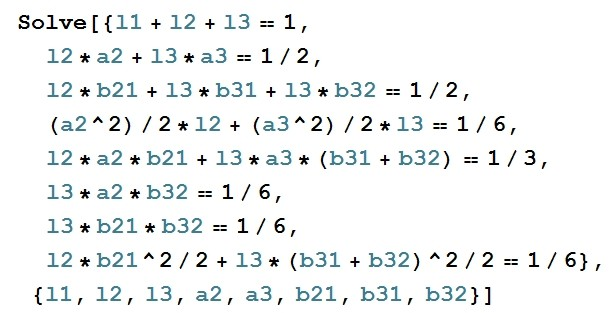
\includegraphics[scale = 0.5]{0.jpg} \\
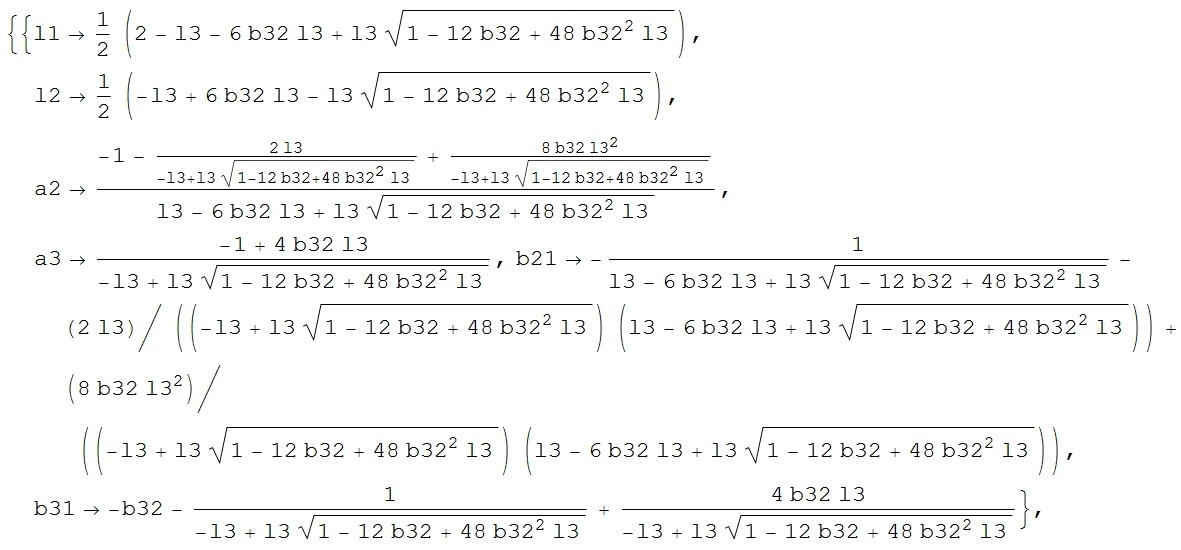
\includegraphics[scale = 0.5]{a.jpg} \\
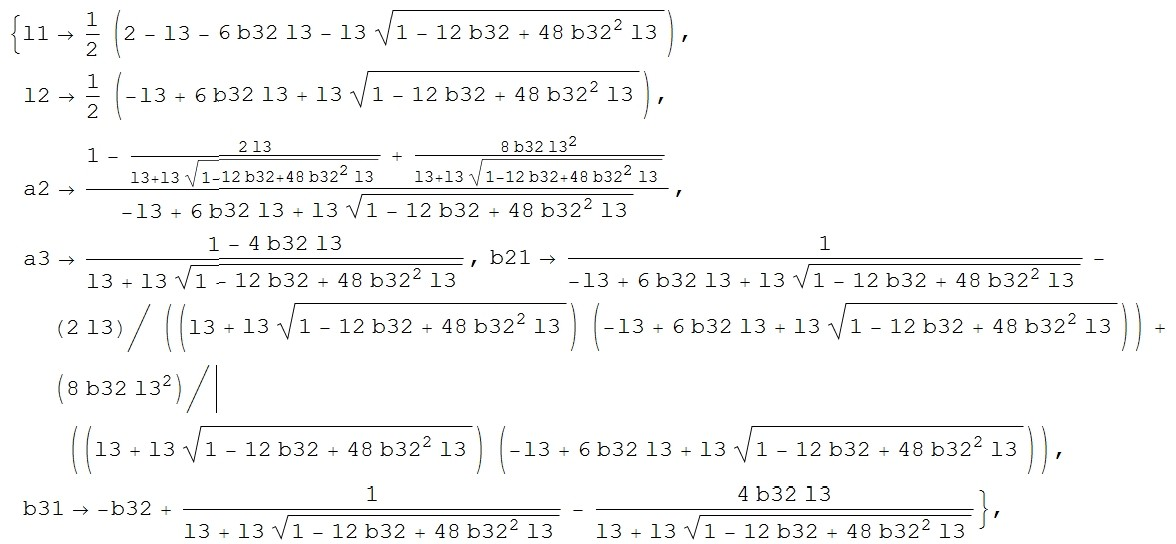
\includegraphics[scale = 0.5]{b.jpg} \\
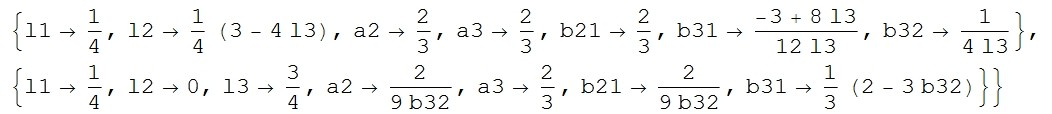
\includegraphics[scale = 0.5]{c.jpg}

我的方程组与未知数一样多,而其他教材上的都有$2$个自由变量。

\section{$8-12$ $8-13$}
这两题很类似。

\subsection{$8-12$}
确定二步方法
\[ y_{n + 1} = \frac{1}{2}(y_n + y_{n - 1}) + \frac{h}{4}(4f_{n + 1} - f_n + 3f_{n - 1}) \]
的局部截断误差主项和阶 \\

我的解法: \\
由于
\[ y_{n - 1} = y - hy' + \frac{h^2}{2}y'' - \frac{h^3}{6}y''' + \frac{h^4}{24}y^{(4)} + O(h^5) \]

\[ f_n = y' \]

\[
\begin{aligned}
f_{n + 1} &= y'(x_n + h) \\
&= y' + hy'' + \frac{h^2}{2}y''' + \frac{h^3}{6}y_{(4)} + \frac{h^4}{24}y^{(5)} + O(h^5)
\end{aligned}
\]

\[
\begin{aligned}
f_{n - 1} &= y'(x_n - h) \\
&= y' - hy'' + \frac{h^2}{2}y''' - \frac{h^3}{6}y_{(4)} + \frac{h^4}{24}y^{(5)} + O(h^5)
\end{aligned}
\]

故
\[
\begin{aligned}
y_{n + 1} &= y_n + \left( -\frac{1}{4} + 1 + \frac{3}{4} - \frac{1}{2} \right)h^2y' + \left( 1 - \frac{3}{4} + \frac{1}{4} \right)h^3y'' + \left( \frac{1}{2} + \frac{3}{4}\frac{1}{2} - \frac{1}{6}\frac{1}{2} \right)h^4y''' + O(h^4) \\
&= y + hy' + \frac{h^2}{2}y'' + \frac{19}{24}h^3y''' + O(h^4)
\end{aligned}
\]

而
\[
\begin{aligned}
y(x_{n + 1}) &= y(x_n + h) \\
&= y + hy' + \frac{h^2}{2}y'' + \frac{h^3}{6}y''' + O(h^4)
\end{aligned}
\]

故截断误差为
\[
\begin{aligned}
y(x_{n + 1}) - y_{n + 1} &= \left(\frac{19}{24} - \frac{1}{6}\right)h^3y''' + O(h^4) \\
&= \frac{5}{8}h^3y''' + O(h^4) \\
&= O(h^3)
\end{aligned}
\]

\subsection{$8-13$}
试求系数$\alpha$,$\beta_0$,$\beta_1$,使二步方法
\[ y_{n + 1} = \alpha(y_n + y_{n + 1}) + h(\beta_0f_n + \beta_1f_{n - 1}) \]
的局部截断误差阶尽可能的高,并写出截断误差主项 \\

我的解法(直接利用上题中算的):
\[ y_{n + 1} = (\alpha + \alpha)y_n + (\beta_0 + \beta_1 - \alpha)hy' + \left(-\beta_1 + \frac{\alpha}{2}\right)h^2y'' + \left(\frac{\beta_1}{2} - \frac{\alpha}{6}\right)h^3y''' + O(h^4) \]

与$y(x_{n + 1})$比较,有方程
\[
\begin{cases}
2\alpha = 1 \\
\beta_0 + \beta_1 + \alpha = 1 \\
-\beta_1 + \dfrac{\alpha}{2} = 1
\end{cases}
\]

解得
\[
\begin{cases}
\alpha = \dfrac{1}{2} \\
\beta_0 = \dfrac{7}{4} \\
\beta_1 = -\dfrac{1}{4}
\end{cases}
\]

同理,截断误差为
\[
\begin{aligned}
\left( \frac{\beta_1}{2} - \frac{\alpha}{6} \right)h^3y''' + O(h^4) &= \left\{\left[ \frac{1}{2}\left( -\frac{1}{4} \right) - \frac{1}{6}\frac{1}{2} \right] - \frac{1}{6}\right\}h^3y''' + O(h^4) \\
&= -\frac{3}{8}h^3y''' + O(h^4)
\end{aligned}
\]

\end{CJK*}
\end{document}